\documentclass{standalone}
\usepackage{tikz}
\usetikzlibrary{shapes, arrows.meta}

\begin{document}
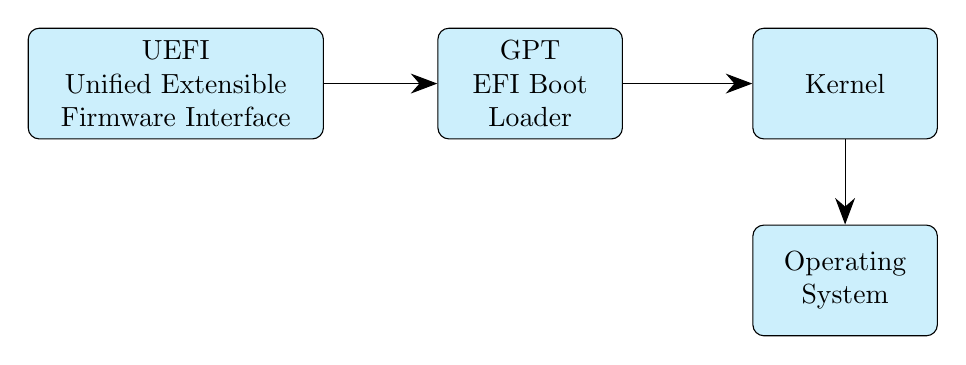
\begin{tikzpicture}[node distance=4.5cm, auto]

    % Styles
    \tikzstyle{block} = [rectangle, draw, fill=cyan!20, 
        text width=6em, text centered, rounded corners, minimum height=4em]
    \tikzstyle{line} = [draw, -{Stealth[scale=2.0]}]

    % Nodes
    \node [block, text width= 10em] (uefi) {UEFI\\Unified Extensible Firmware Interface};
    \node [block, right of=uefi] (gpt) {GPT\\EFI Boot Loader};
    \node [block, right of=gpt, node distance=4cm] (kernel) {Kernel};
    \node [block, below of=kernel, node distance=2.5cm] (os) {Operating System};

    % Paths
    \path [line] (uefi) -- (gpt);
    \path [line] (gpt) -- (kernel);
    \path [line] (kernel) -- (os);

\end{tikzpicture}
\end{document}
